%%%%%%%%%%%%%%%%%%%%%%%%%%%%%%%%%%%%%%%%%
% Beamer Presentation
% LaTeX Template
% Version 1.0 (10/11/12)
%
% This template has been downloaded from:
% http://www.LaTeXTemplates.com
%
% License:
% CC BY-NC-SA 3.0 (http://creativecommons.org/licenses/by-nc-sa/3.0/)
%
%%%%%%%%%%%%%%%%%%%%%%%%%%%%%%%%%%%%%%%%%

%----------------------------------------------------------------------------------------
%	PACKAGES AND THEMES
%----------------------------------------------------------------------------------------

\documentclass{beamer}

\mode<presentation> {

% The Beamer class comes with a number of default slide themes
% which change the colors and layouts of slides. Below this is a list
% of all the themes, uncomment each in turn to see what they look like.

%\usetheme{default}
%\usetheme{AnnArbor}
%\usetheme{Antibes}
%\usetheme{Bergen}
%\usetheme{Berkeley}
%\usetheme{Berlin}
%\usetheme{Boadilla}
%\usetheme{CambridgeUS}
%\usetheme{Copenhagen}
%\usetheme{Darmstadt}
%\usetheme{Dresden}
%\usetheme{Frankfurt}
%\usetheme{Goettingen}
%\usetheme{Hannover}
%\usetheme{Ilmenau}
%\usetheme{JuanLesPins}
%\usetheme{Luebeck}
\usetheme{Madrid}
%\usetheme{Malmoe}
%\usetheme{Marburg}
%\usetheme{Montpellier}
%\usetheme{PaloAlto}
%\usetheme{Pittsburgh}
%\usetheme{Rochester}
%\usetheme{Singapore}
%\usetheme{Szeged}
%\usetheme{Warsaw}

% As well as themes, the Beamer class has a number of color themes
% for any slide theme. Uncomment each of these in turn to see how it
% changes the colors of your current slide theme.

%\usecolortheme{albatross}
%\usecolortheme{beaver}
%\usecolortheme{beetle}
%\usecolortheme{crane}
%\usecolortheme{dolphin}
%\usecolortheme{dove}
%\usecolortheme{fly}
%\usecolortheme{lily}
%\usecolortheme{orchid}
%\usecolortheme{rose}
%\usecolortheme{seagull}
%\usecolortheme{seahorse}
%\usecolortheme{whale}
%\usecolortheme{wolverine}

%\setbeamertemplate{footline} % To remove the footer line in all slides uncomment this line
%\setbeamertemplate{footline}[page number] % To replace the footer line in all slides with a simple slide count uncomment this line

%\setbeamertemplate{navigation symbols}{} % To remove the navigation symbols from the bottom of all slides uncomment this line
}

\usepackage{graphicx} % Allows including images
\usepackage[absolute, overlay]{textpos}
\usepackage{booktabs} % Allows the use of \toprule, \midrule and \bottomrule in tables
\usepackage{tikz}
\usepackage{amsmath}
\usepackage{animate}
\usepackage{media9}
\usepackage{algorithm,algorithmic}

\usetikzlibrary{positioning,calc,backgrounds,shapes}

\usepackage[labelformat=empty]{caption}
\captionsetup{compatibility=false}

\tikzset{My Arrow Style/.style={single arrow, fill=red!30, anchor=base, align=center,text width=4cm}}
\newcommand{\arrowthis}[2][]{\tikz[baseline] \node [My Arrow Style,#1] {#2};}


\tikzset{My Speech Style/.style={ellipse callout, fill=red!50, anchor=base, align=center,text width=2.8cm}}
\newcommand{\speechthis}[2][]{
    \tikz[baseline]{\node[My Speech Style, #1]{#2};}
}%Ea
\newcommand{\source}[1]{\begin{textblock*}{4cm}(8.7cm,8.2cm)
        \begin{beamercolorbox}[ht=0.5cm,right]{framesource}
        \usebeamerfont{framesource}\usebeamercolor[fg]{framesource} Source: {#1}
        \end{beamercolorbox}
    \end{textblock*}
}
\newcommand{\norm}[1]{\left\lVert#1\right\rVert}

%----------------------------------------------------------------------------------------
%	TITLE PAGE
%----------------------------------------------------------------------------------------

\title[Bitdefender, University of Bucharest]{Introduction to Lattice Based Cryptography}
% The short title appears at the bottom of every slide, the full title is only on the title page
%An Immediate Multi-Party Generalization of ID-NIKE from Constrained PRF
\author[D.A.Rotaru]{Drago\c{s} Alin Rotaru} % Your name
\institute[Bitdefender, Unibuc] % Your institution as it will appear on the bottom of every slide, may be shorthand to save space
{
Bitdefender Romania,
University of Bucharest\\ % Your institution for the title page
% \medskip
% \textit{ruxandra.olimid@fmi.unibuc.ro, r.dragos0@gmail.com} % Your email address
}
\date{October 21, 2015} % Date, can be changed to a custom date

\begin{document}

\begin{frame}
\titlepage % Print the title page as the first slide
\end{frame}


%----------------------------------------------------------------------------------------
%	PRESENTATION SLIDES
%----------------------------------------------------------------------------------------

%------------------------------------------------
\section{Outline} % Sections can be created in order to organize your presentation into discrete blocks, all sections and subsections are automatically printed in the table of contents as an overview of the talk
%------------------------------------------------

\begin{frame}
    \frametitle{Outline} % Table of contents slide, comment this block out to remove it
    \begin{itemize}
        \item What is a lattice?
        \item Lattices in practice.
        \item Examples of hard problems on lattices.
        \item (Known) Algorithms for solving hard problems on lattices.
        \item Cyclic lattices and the NTRU cryptosystem.
    \end{itemize}
\end{frame}

%------------------------------------------------

%TODO: Insert slides about signatures, post quantum, FHE, Obfuscation
\section{Basic facts about lattices}
\begin{frame}
    \frametitle{What is a lattice? v.1}
    \only<1-> {
        Short Answer: A grid.
        \begin{figure}
            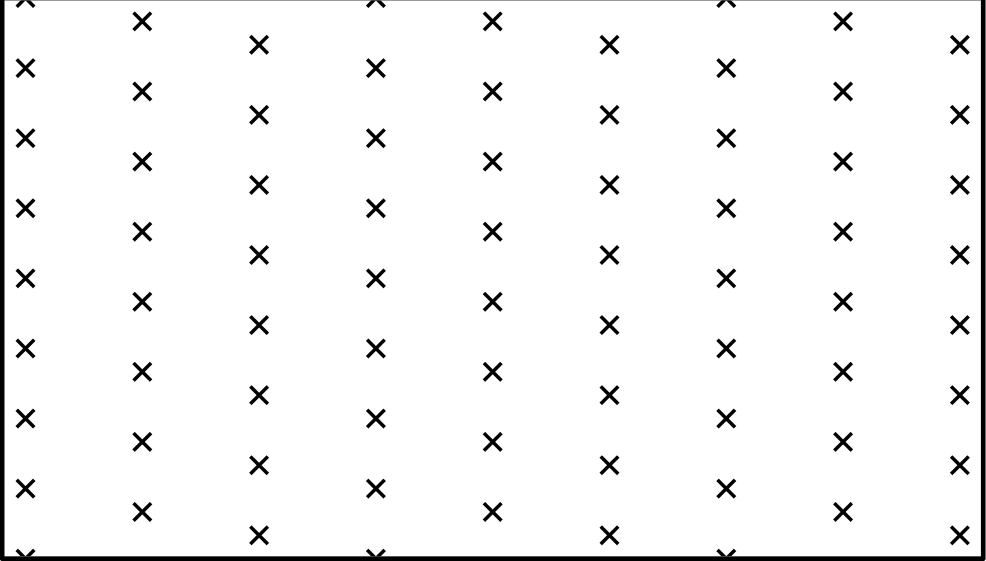
\includegraphics[width=7cm,height=7cm,keepaspectratio]{img/latticer2.png}
            \caption{Lattice in $R^2$}
        \end{figure}
    }
\end{frame}

% TODO: Write about the tradeoff between security proofs and practical systems
% 
\begin{frame}
    \frametitle{What is a lattice? v.2}
    \begin{itemize}
        \item The set of all linear integers combinations by some vectors in $R^m$.
        \pause \item Given $n$ linearly independent vectors $\mathbf{b}_1, \mathbf{b}_2, \dots, \mathbf{b}_n \in \mathbb{R}^m$ the lattice generated by them is $\mathcal{L}(\mathbf{b}_1, \mathbf{b}_2, \dots, \mathbf{b}_n) = \{ \sum\nolimits{}{x_ib_i} , x_i \in \mathbb{Z}\}$.
        \pause \item We call $\mathbf{b}_1, \mathbf{b}_2, \dots \mathbf{b}_n$ the basis of $\mathcal{L}$.
        \pause \item Rewrite the definition as $\mathcal{L} = Bx$ where $B$ has $n$ columns: $\mathbf{b}_1, \mathbf{b}_2, \dots, \mathbf{b}_n$.

    \end{itemize}
\end{frame}

%TODO: Insert slide about how a lattice can have multiple bases
%Done.

\begin{frame}
    \frametitle{Lattice Basis}
    \begin{figure}
            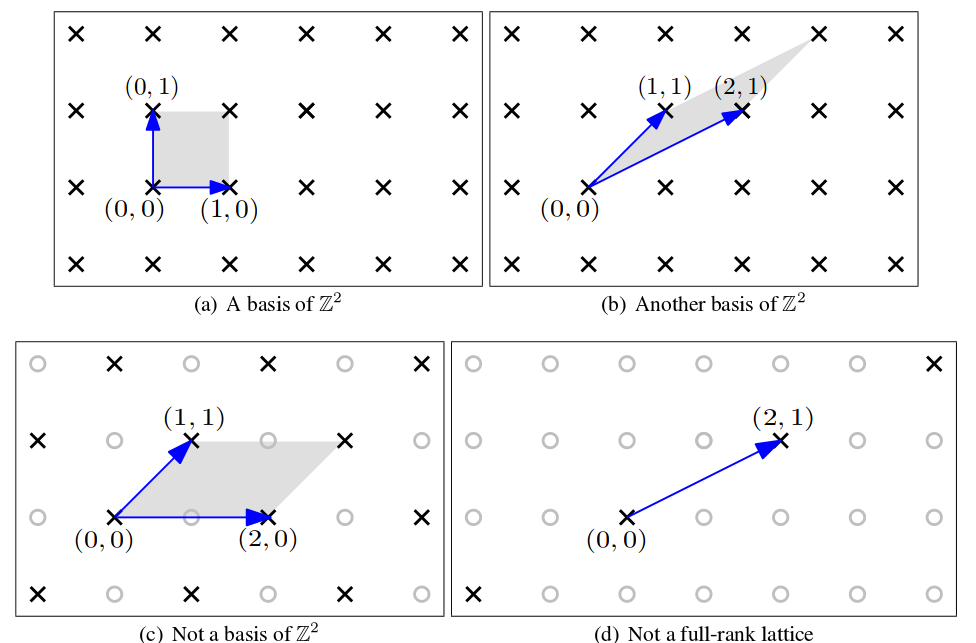
\includegraphics[width=10cm,height=10cm,keepaspectratio]{img/lattice_bases.png}
            \caption{Different bases - Source: Regev course}
        \end{figure}
\end{frame}
\begin{frame}
    \frametitle{Lattice Basis}
    \begin{block}<1->{Fact}
        $\mathcal{L}(B) = \mathcal{L}(B')$ if and only if there exists an unimodular integer matrix $U \in \mathbb{Z}^{nxn}$ such that $B = B'U$.
    \end{block} 
    \begin{itemize}
        \pause \item Because $U$ is unimodular, $det(U) = \pm 1$.
        \pause \item So what?
        \pause \item $det(B)$ it's invariant over the choice of basis. Denote $det(\mathcal{L}) := |det(B)|$.
        \pause \item $det(\mathcal{L})$ is also called the fundamental volume of $\mathcal{L}$.
        \pause \item Determinant of a lattice is inverse proportional to its density.
        % TODO: Insert a figure of how the det(L) behaves as it the points of the lattices are approaching.
        % Actually, as the determinant goes to 0 then the lattice points are very closed; Vol(K) / Det(L) = 
    \end{itemize}
\end{frame}

\begin{frame}
    \frametitle{Succesive minima}
    \begin{block}<1->{Shortest Vector}
        $\lambda_1(\mathcal{L}) = min \{ \norm{x} : x \in \mathcal{L}, x \neq 0 \} $
    \end{block}
    % observe that if x is the shortest vector, then -x is also a SV.
    \begin{block}<2->{Succesive minima}
        $\lambda_i(\mathcal{L}) = min \{ r : dim( span( \mathcal{L} \cap B(0, r) )) \geq i \} $
    \end{block}
    \begin{block}<3->{Upper bounds for $\lambda_1(\mathcal{L})$}
        For any lattice of dimension $n$, $\lambda_1(\mathcal{L}) \le \sqrt{n}(det(\mathcal{L}))^{ 1/n }$.
    \end{block}
    \begin{itemize}
        \pause \pause \pause \item Unfortunately, no constructive proof.
        \pause \item Also, a loose bound. Think about the lattice generated in $\mathbb{R}^2$ by 
        $\begin{bmatrix}
        0 & \epsilon \\
        1/e & 0 \\
        \end{bmatrix}$
    \end{itemize}
\end{frame}

\begin{frame}
    \frametitle{Dream world: Gram-Schmidt for Lattices}
    \begin{itemize}
        \item It would be great to have a basis $\mathbf{b}_1 = \lambda_1(\mathcal{L}), \mathbf{b}_2 = \lambda_2(\mathcal{L}), \dots, \mathbf{b}_n = \lambda_n(\mathcal{L})$.
        \pause \item Because the fundamental volume of $\mathcal{L}$ is invariant over the change of basis, short and orthogonal are related notions.
        \pause \item Solution: Let's apply Gram-Schmidt to a lattice basis!
        \pause \item What?
    \end{itemize}
\end{frame}


\begin{frame}
    \frametitle{Gram-Schmidt Ortogonalization}
        \begin{figure}
            \includegraphics[width=5cm,height=4cm,keepaspectratio]{img/Gram–Schmidt_process.png}
            \caption{Ortogonalizations of $2$ vectors in $\mathbf{R}^2$; source: Wiki}
        \end{figure}

    \begin{itemize}
        \item Input: Basis $\{ \mathbf{b}_1, \mathbf{b}_2, \dots , \mathbf{b}_n \} $
        \pause \item Output: $\tilde{\mathbf{b}}_1, \tilde{\mathbf{b}}_2, \dots, \tilde{\mathbf{b}}_n$, such that $ \langle \tilde{\mathbf{b}}_i, \tilde{\mathbf{b}}_j \rangle = 0, i \neq j$ 
        \pause \item Define the projection operator: $proj_{u}(v) = \frac{\langle v, u \rangle}{\langle u, u \rangle}u$.
        \pause \item $\tilde{\mathbf{b}}_1 = \mathbf{b}_1, \tilde{\mathbf{b}}_2 = \mathbf{b}_2 - proj_{\tilde{\mathbf{b}}_1}({\mathbf{b}}_2)$ and so on.
        \pause \item $\tilde{\mathbf{b}}_i = \mathbf{b}_i - \sum_{j=1}^{i-1}{\frac{\langle \tilde{\mathbf{b}}_j, \mathbf{b}_i \rangle}{\langle \tilde{\mathbf{b}}_j, \tilde{\mathbf{b}}_j \rangle} \tilde{\mathbf{b}}_j}$.
        \pause \item Cool! Now plug-in a lattice and find an orthogonal basis! What is wrong with this approach?
    \end{itemize}
\end{frame}

\begin{frame}
    \frametitle{Gram-Schmidt for Lattices - LLL Reduction}
    By changing the basis, we change the spanned lattice.
    \begin{figure}
            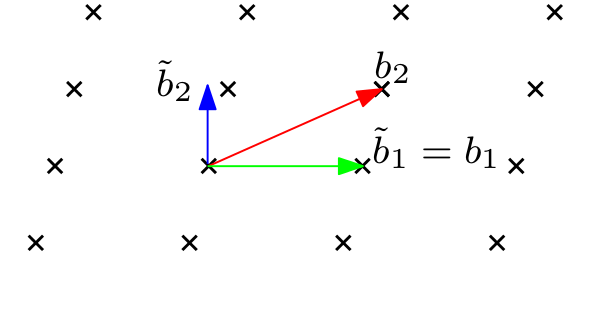
\includegraphics[width=5cm,height=4cm,keepaspectratio]{img/gram-schmidt.png}
            \caption{Ortogonalizations of $2$ lattice vectors in $\mathbf{R}^2$; source: Regev O. course}
        \end{figure}

    \textbf{Solution: Round the projection to the nearest integer!}
\end{frame}

\begin{frame}
    \frametitle{Gram-Schmidt for Lattices - LLL Reduction}
    \begin{block}<1->{LLL Reduction}
        Input: Basis $\{ \mathbf{b}_1, \mathbf{b}_2, \dots , \mathbf{b}_n \} $
        Output: $\delta$-LLL reduced basis.
    \end{block}
    \begin{algorithm}[H]
    \begin{algorithmic}[1]
    %Compute $\tilde{\mathbf{b}}_1, \tilde{\mathbf{b}}_2, \dots, \tilde{\mathbf{b}}_n$ 
    \FOR{$i=1$ to $N$}
    \FOR{$j=i-1$ to $1$}
    \STATE $b_i =$ $b_i - \lfloor c_{i, j} \rceil b_j$, $c_{i, j} = \frac{\langle \tilde{\mathbf{b}}_j, \mathbf{b}_i \rangle}{\langle \tilde{\mathbf{b}}_j, \tilde{\mathbf{b}}_j \rangle}$
    \ENDFOR

    \STATE \emph{Swap Step}:
    \IF {$\exists i$ s.t. $\delta$} \RETURN false
    \ENDIF

    \ENDFOR

    \end{algorithmic}
    \caption{pseudocode for the calculation of }
    \label{alg:seq}
    \end{algorithm}

\end{frame}
%TODO: Not all problems related to lattices are hard. Insert a slide about easy problems. Membership of a vector into a lattice. Check if 2 bases are equivalent.
\begin{frame}
    \frametitle{testing}
    \begin{center}
    $Bx = 
      \begin{bmatrix}
            | & | & \cdots & |\\
            b_1 & b_2 & \cdots & b_n \\
            | & | & \cdots & |
     \end{bmatrix}
     \begin{bmatrix}
        x_1\\
        x_2\\
        \vdots \\
        x_n 
    \end{bmatrix}$
    \end{center}
\end{frame}


\begin{frame}
\Huge{\centerline{Thank you!}}
\end{frame}
\end{document}
